\documentclass[10pt,a4paper]{article}
\usepackage[utf8]{inputenc}
\usepackage{amsmath}
\usepackage{amsfonts}
\usepackage{amssymb}
\usepackage{graphicx}
\usepackage{fancyhdr}
\usepackage{xcolor}
\usepackage{xparse}
\usepackage[french]{babel}
\usepackage[left=2cm,right=2cm,top=2cm,bottom=2cm]{geometry}
\pagestyle{fancy}

\NewDocumentCommand{\framecolorbox}{oommm}
 {% #1 = width (optional)
  % #2 = inner alignment (optional)
  % #3 = frame color
  % #4 = background color
  % #5 = text
  \IfValueTF{#1}
   {%
    \IfValueTF{#2}
     {\fcolorbox{#3}{#4}{\makebox[#1][#2]{#5}}}
     {\fcolorbox{#3}{#4}{\makebox[#1]{#5}}}%
   }
   {\fcolorbox{#3}{#4}{#5}}%
 }

\renewcommand{\headrulewidth}{1pt}
\fancyhead[C]{} 
\fancyhead[L]{INF7235 - Devoir \#1}
\fancyhead[R]{Reynaud Nicolas}

\renewcommand{\footrulewidth}{1pt}
\fancyfoot[C]{\LaTeX} 
\fancyfoot[L]{\small\hspace{15pt}\emph{Imprimé le : \today}}
\fancyfoot[R]{Page \thepage}

\begin{document}

\section{Description du problème}

\indent Le problème que j'ai choisi est le jeu de la vie. Dans ce dernier, l'élément à parallélisé parait assez évidant. \\
En effet, dans ce jeu le principe est de partir d'une grille de N x M (N $>$ 0 \& M $>$ 0), dans laquelle les cellules peuvent se trouver seulement dans deux états. Une cellule est soit morte, soit vivante. 
Le principe du jeu est alors, à partir de cette grille et d'une série de règle très simple de calculer la grille suivante.
Le jeu de la vie n'a pas de but, il s'agit uniquement de faire évoluer un automate cellulaire au cours du temps.\\

Les règles se bas sur un calcule en fonction du nombre de voisin d'une cellule; ainsi une cellule ayant 3 cellules vivante à coté d'elle sera vivante à l'étape d'après, une cellule ayant moins de 2 cellules en vie ou plus de 3 en vie à coté d'elle mourra, et enfin une cellule ayant exactement 2 cellules vivante à côté d'elle restera dans le même état. Ainsi à partir de ces règles il nous faut calculer la grille suivante. \\

Ainsi en suivant ces règles la grille suivante n'a pas d'interdépendance lors de son calcule (nous n'avons pas besoin de savoir quoi que ce soit de la seconde grille pour la calculer). Ainsi la parallélisation parait assez évidente. Il suffit de demander à chaque threads de calculer une partie de la grille. \\
Bien entendu cette partie ne doit pas être trop petite, en effet si par exemple nous choisissions de prendre une unique cellule pour chaque threads, il nous faudrait alors N x M threads.

\section{Les approches}
La première approche fait et bien entendu celle en séquentiel, afin d'avoir une version de base servant de comparaison. \\

Je suis ensuite passé deux version multithread. Comme indiqué précédemment une approche utilisant un thread pour une action n'était pas viable, une action étant de prendre une case, compter ces voisin puis calculer le nouvelle état d'une cellule. \\

J'ai donc opté pour une division de la grille en colonne. \\

Soit une grille de N x M ou N est le nombre de ligne et M le nombre de colonne, et T le nombre de thread.
\begin{itemize}
    \item En granularité fine, chaque thread traite une colonne de la grille et calcule le résultat de celle ci. Il faudra donc M threads pour une grille de N x M,  \\
    \underline{Exemple} : Si il n'y a que un thread celui ci traitera à lui seul les M colonnes à la suite mais en les traitant comme une colonne à chaque fois et non un bloc de M colonne.\\
    
    \item En granularité grossière, j'ai opté pour une division en colonne continue. \\
    Ainsi chaque thread traite M / T colonnes. Ici toutes les colonnes seront donc traité en parallèle peut importe le nombre de thread. \\
    \underline{Exemple} : Si il n'y a que un thread il traitera à lui seul les M colonnes à la suite en un seul appel.
\end{itemize}
\hfill\break
\underline{A noter} : Les méthodes avec des threads n'utiliseront que le nombre de thread nécessaire, ainsi si on demande au programme d'utiliser 1000 threads pour une grille de 100 x 100, seule 100 threads seront réellement utilisé. \\

Au départ j'étais d'abord partie dans la simplicité ainsi à chaque "tick" de game ( un tick étant une évolution complète de la grille ); les threads était crée le temps du traitement puis détruit à la fin du traitement ( et donc à la fin du tick). 
Il était ensuite recrée pour le tick suivant puis était arrêté à la fin de leurs traitement et ainsi de suite. \\

Cette méthode n'étant pas du tout optimale j'ai modifié la méthode de traitement, au départ du programme T threads sont créé, puis par la suite deux cas peuvent se produire :
\begin{itemize}
    \item Au premier tick une liste de tache est crée, et si il y a assez de thread pour toutes les traiter côte à cote, et donc jamais changer de taches, les taches ne sont alors plus crée et chaque thread gardera sa tache jusqu'à la fin du programme.
    \item Dans un autre cas, si il n'y a pas assez de thread pour que ceci puissent garder leurs taches, celle ci sont alors crée à chaque tick de jeu, puis chaque thread pioche dans celle liste jusqu'à ce qu'elle soit vidée. Ainsi les threads qui finissent leurs taches ne restent pas à rien faire si il reste des taches.
\end{itemize}

\section{Les tests}
Pour les stratégies de tests j'ai deux stratégies différente, la première avec \framecolorbox[1.7cm]{white}{black!20}{make tests} permet de lancer des tests avec des grilles prédéfinie, grilles dont les résultats sont connu en avance, il s'agit principalement de grille qui n'évolue pas ou peu au cours du temps. \\

Ainsi chaque tests se compose de la façon suivante : 
\begin{itemize}
    \item Prendre un des tests de la liste.
    \item Calculer la grille de fin et la sauvegarder dans un fichier.
    \item Comparer la grille généré à celle qui était prévue.
    \item Indiqué si un problème ou non c'est passé.
    \item Si un problème à survenue indiqué les différences entre les deux (2) grilles.
\end{itemize}

\hfill \break

La seconde stratégie de test, est lancée avec la commande \framecolorbox[2.5cm]{white}{black!20}{make tests-rand}, \\
ou la commande \framecolorbox[4.6cm]{white}{black!20}{make tests-rand TOTAL=X}, ou X est le nombre de tests à faire, par défaut X=5. \\

Lors de ces tests une grille est générée aléatoirement, ensuite cette grille évolue un nombre Y de fois; avec 0 $<$ Y $<$ 100, la valeur 100 est une valeur fixée par la constante MAX\_ITERATION du fichier ./Script/test\_random.sh. \\

L'évolution du jeu est dans un premier temps effectué par le programme séquentiel qui est la version qui nous servira de base pour comparer avec les versions créée par les versions avec des threads. \\
Une fois cette génération séquentiel terminée, une première version du programme est lancé en utilisant les threads avec une granularité fine, puis une autre avec une granularité grossière. Le nombre de thread T'; avec 0 $<$ T' $<$ 20, la valeur 20 est fixée par une constante MAX\_THREAD dans le fichier ./Script/test\_random.sh. \\

Les versions généré par les versions du programme avec les threads sont alors comparées avec la version générée de façon séquentiel, si une différence est détectée celle-ci est affichée. \\	

\underline{A noter : } A la fin des programmes de tests une chaine de caractère est affichée sous la forme : ".\#...." par exemple, ou "." signifie qu'un test est passé avec succès, "\#" signifiant que le tests à échoué. Ainsi ici le tests deux (2) aurait échoué.

\section{Résultats expérimentaux}

Les résultats expérimentaux pour les valeurs suivantes : 10, 50, 100, 500, 1000 \& 2000. \\
\begin{figure}[h]
  \centering
  \begin{minipage}[b]{0.49\textwidth}
	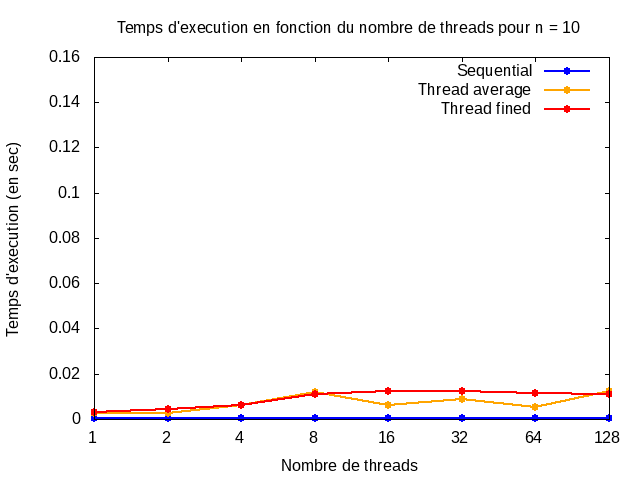
\includegraphics[width=\textwidth]{./Time/size_10_time.png}
    \caption{Temps d'exécution pour une grille de 10 x 10}
  \end{minipage}
  \hfill
  \begin{minipage}[b]{0.49\textwidth}
    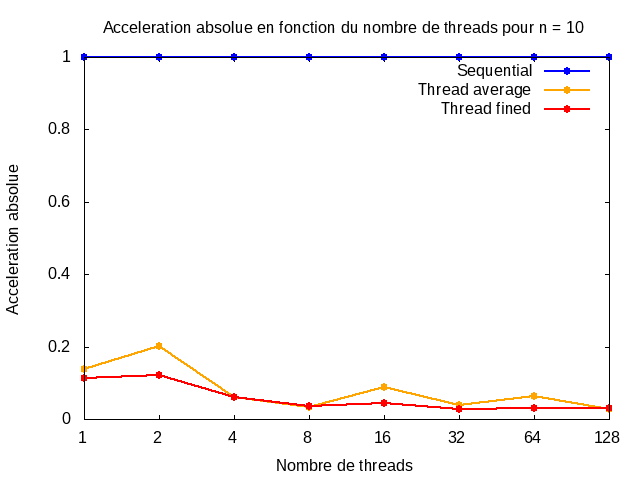
\includegraphics[width=\textwidth]{./Time/size_10_acceleration.png}
    \caption{Accélération absolue pour une grille de 10 x 10}
  \end{minipage}
\end{figure}
\hfill \break
Ces premiers résultats ne sont pas très concluant, en effet, on remarque une accélération très faible pour les deux programmes avec des threads. Pour cause, dans ce problème il n'y a aucun intérêt de lancer  des threads qui sont très couteux en ressource pour effectué des calcules sur une grille de 10 x 10.

Ainsi ici on remarque que les temps d'exécutions sont presque les mêmes, même si les versions avec des threads sont plus lentes ( dût au fait du lancement des threads ).\\
On remarque également une stabilisation des temps à partir de 8 threads, en effet au dessus de 10 threads le nombre de thread demandé est ramené à 10.
\begin{figure}[h]
  \centering
  \begin{minipage}[b]{0.49\textwidth}
	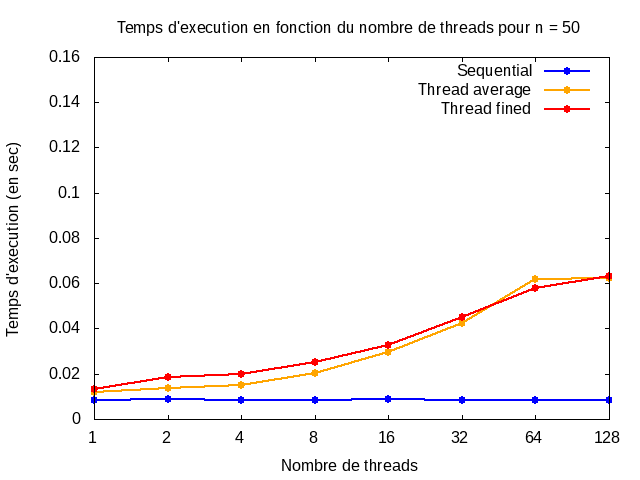
\includegraphics[width=\textwidth]{./Time/size_50_time.png}
    \caption{Temps d'exécution pour une grille de 50 x 50}
  \end{minipage}
  \hfill
  \begin{minipage}[b]{0.49\textwidth}
    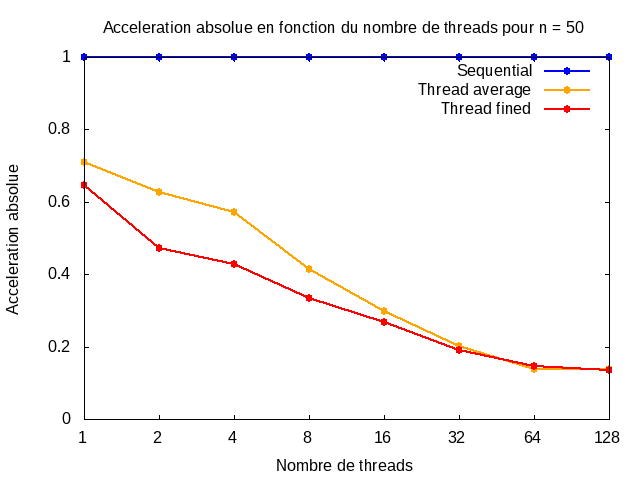
\includegraphics[width=\textwidth]{./Time/size_50_acceleration.png}
    \caption{Accélération absolue pour une grille de 50 x 50}
  \end{minipage}
\end{figure}
Dans ces mesures, on remarque que le temps d'exécution augmente proportionnellement au nombre de thread, en effet il faut de plus en plus de temps pour crée un nombre conséquent de thread.\\
Ici l'accélération est un peu mieux que dans l'exemple précédent, cependant je test est encore trop petit pour parallélisé les calcules.\\

\begin{figure}[h]
  \centering
  \begin{minipage}[b]{0.49\textwidth}
	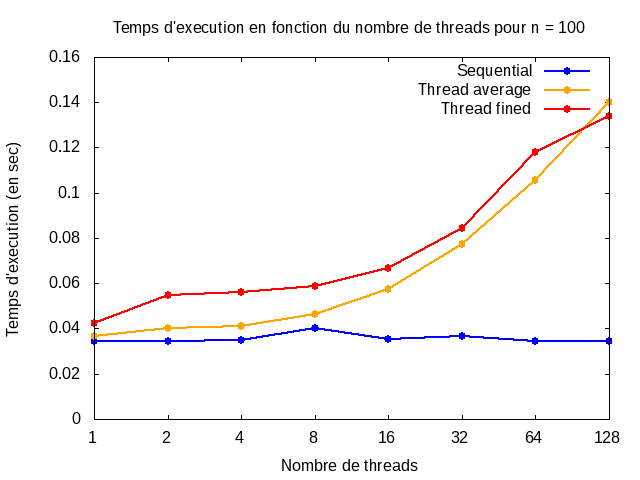
\includegraphics[width=\textwidth]{./Time/size_100_time.png}
    \caption{Temps d'exécution pour une grille de 100 x 100}
  \end{minipage}
  \hfill
  \begin{minipage}[b]{0.49\textwidth}
    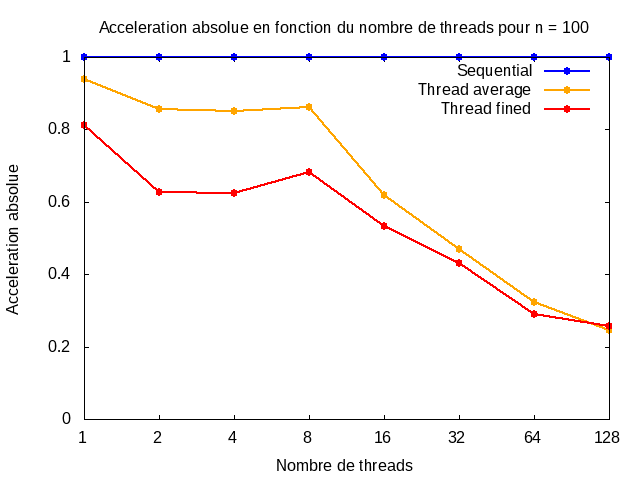
\includegraphics[width=\textwidth]{./Time/size_100_acceleration.png}
    \caption{Accélération absolue pour une grille de 100 x 100}
  \end{minipage}
\end{figure}

Encore une fois, les temps d'exécutions augmente proportionnellement avec le nombre de thread, ont remarque également que le temps entre la méthode à granularité fine et la granularité grossière est assez grande au début, puis diminue ensuite avec un nombre de thread plus conséquent.\\
En effet, au départ le manque de thread implique donc que un ou plusieurs threads doivent effectué plusieurs taches à la suite dès qu'ils ont fini leurs taches. \\
Cependant l'accélération est meilleur sur cette endroit la (dans le cas d'une granularité fine). \\

\newpage
\begin{figure}[h]
  \centering
  \begin{minipage}[b]{0.49\textwidth}
	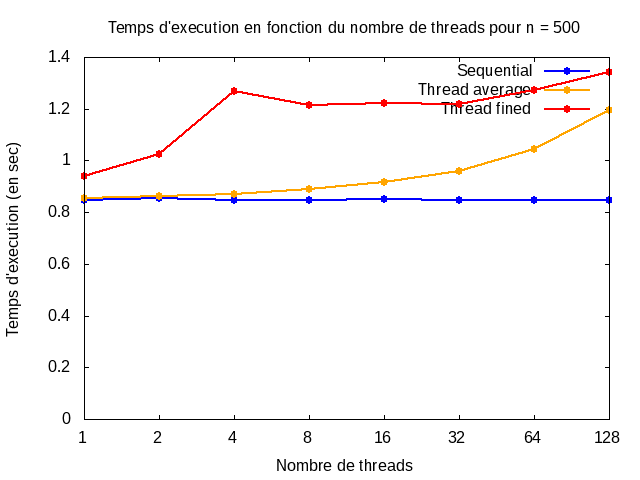
\includegraphics[width=\textwidth]{./Time/size_500_time.png}
    \caption{Temps d'exécution pour une grille de 500 x 500}
  \end{minipage}
  \hfill
  \begin{minipage}[b]{0.49\textwidth}
    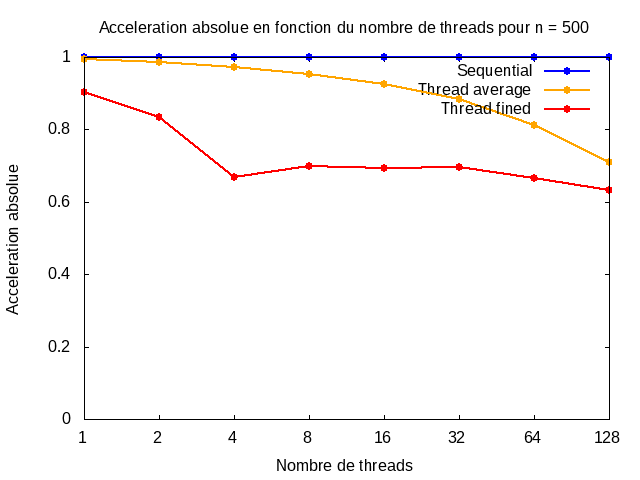
\includegraphics[width=\textwidth]{./Time/size_500_acceleration.png}
    \caption{Accélération absolue pour une grille de 500 x 500}
  \end{minipage}
\end{figure}
Ici on remarque que les temps d'exécution différent de plus en plus entre la granularité fine et grossière, on remarque également que au départ, le temps d'exécution est presque le même entre le temps séquentiel et le temps de la granularité grossière. En effet, sur de tels temps d'exécution le fait de lancer un seul thread est négligeable par rapport au temps total d'exécution.\\
Ainsi sur un tel problème une méthode séquentiel et presque équivalente à un problème-multi thread (ou avec peu de thread) avec une granularité grossière. \\

\begin{figure}[h]
  \centering
  \begin{minipage}[b]{0.49\textwidth}
	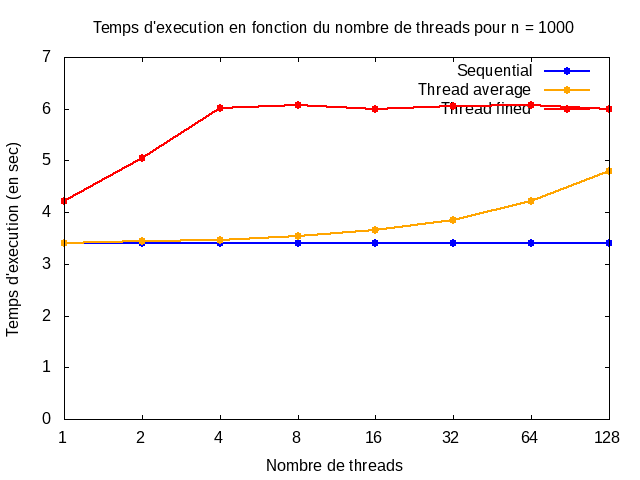
\includegraphics[width=\textwidth]{./Time/size_1000_time.png}
    \caption{Temps d'exécution pour une grille de 1000 x 1000}
  \end{minipage}
  \hfill
  \begin{minipage}[b]{0.49\textwidth}
    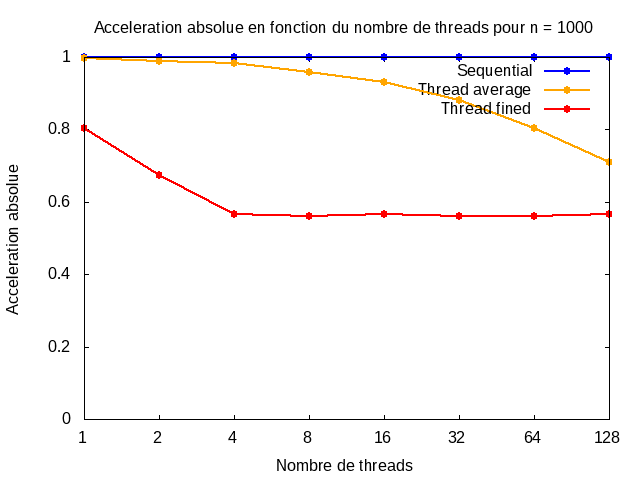
\includegraphics[width=\textwidth]{./Time/size_1000_acceleration.png}
    \caption{Accélération absolue pour une grille de 1000 x 1000}
  \end{minipage}
\end{figure}

Avec ce teste, on remarque des résultats beaucoup plus concluant, on remarque notamment une augmentation énorme du temps d'exécution avec la méthode à granularité fine. En effet, il n'y a pas assez de thread pour traiter les 1000 taches en parallèle, obligeant ainsi chaque thread à, à chaque tick, reprendre une tache dans la liste des taches jusqu'à vidé celle ci. Ainsi il faut que les T premières taches soit finie avant de passer au T' taches suivantes.\\

On remarque également une "fusion" avec un petit nombre de thread des courbes de la version séquentiel et celle à granularité grossière. En effet, le temps pris pour la création des taches / threads sont redue mineur par rapport au temps total d'exécution. \\
Cette remarque s'applique également pour l'accélération absolue, ainsi on remarque une très bonne accélération avec la méthode multi-thread à granularité grossière étant donné qu'il revient pratiquement au problème séquentiel (avec la création des threads).


\begin{figure}[h]
  \centering
  \begin{minipage}[b]{0.49\textwidth}
	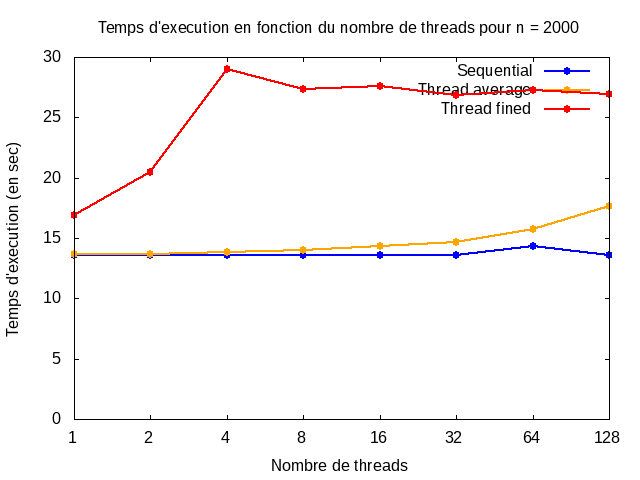
\includegraphics[width=\textwidth]{./Time/size_2000_time.png}
    \caption{Temps d'exécution pour une grille de 2000 x 2000}
  \end{minipage}
  \hfill
  \begin{minipage}[b]{0.49\textwidth}
    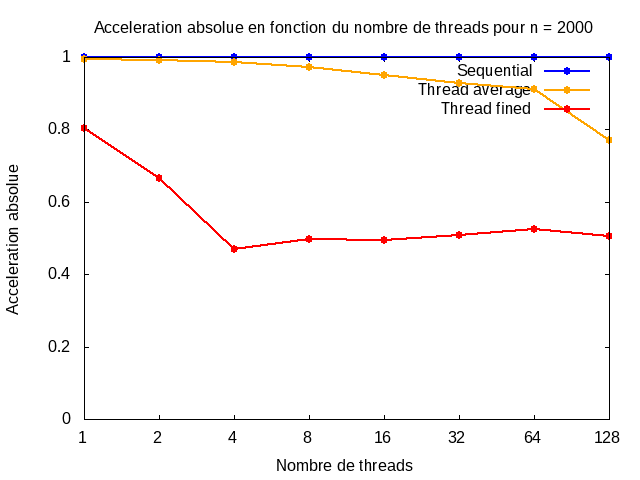
\includegraphics[width=\textwidth]{./Time/size_2000_acceleration.png}
    \caption{Accélération absolue pour une grille de 2000 x 2000}
  \end{minipage}
\end{figure}
\newpage
Pour ce test, l'analyse est analogue à celle d'une grille de 1000 x 1000,
seule différence l'augmentation des temps d'exécution.

\underline{A noter} : Je ne suis pas aller au delà d'une grille de 2000 x 2000 étant donné qu'il m'a fallut plus de 40 minutes pour ne serais-ce que généré la grille, puis une autre 30 - 40 aines de minutes pour avoir la création des graphes ( et donc l'exécution complète de toutes les versions du programme).

\section{Conclusion}

En somme, on remarque que la méthode à granularité grossière est plus adapté pour de grande taille de grille. On remarque également qu'il n'y a pas d'intérêt de parallélisé des grilles avec moins de 50 éléments. \\

Enfin, on remarque que la granularité fine n'est pas adapté à ce problème étant donné le temps de tache à effectué par chaque thread, et donc la granularité fine n'a pas d'intérêt dans ce genre de problème.

\section{Fuites mémoires}
Je tenais à faire une section sur ce document présentant une chose où j'ai passé pas mal de temps par conscience professionnelle. Un point qui me tien à cœurs est le fait de n'avoir aucune fuite mémoire dans le cadre normal d'exécution du programme. Mes programmes ont donc tous était testé avec valgrind afin de garantir aucune fuite mémoire.\\

Je vous invite donc à voir le fichier Valgrind\_log présent à la racine du répertoire.

\end{document}
